% =====================================================================
%  OQIM Round 2 plan. Compile with pdfLaTeX (Overleaf default).
%  Figures are in figures/ ; references are in refs.bib and are
%  numbered automatically in the order they are first cited.
% =====================================================================


\documentclass[11pt,letterpaper]{article}

% ---------- Page and fonts ----------
\usepackage[margin=0.75in]{geometry}
\usepackage[T1]{fontenc}
\usepackage{amsmath}
\usepackage{textcomp}
\usepackage{newtxtext,newtxmath}
\usepackage{microtype}

% ---------- Tables, figures, lists ----------
\usepackage[table]{xcolor}
\usepackage{booktabs,tabularx,array}
\usepackage{graphicx}
\usepackage{float}
\usepackage{placeins}
\usepackage{enumitem}
\usepackage{caption}
\usepackage[numbers,sort&compress]{natbib}
\setlength{\bibsep}{0pt plus 0.3ex}
\usepackage{multicol}
% Figures are pre-rendered PDFs in figures/ (made with TikZ/pgfplots).
\usepackage[export]{adjustbox}

% ---------- Headings, footer, links ----------
\usepackage{titlesec}
\usepackage{fancyhdr}
\usepackage{xurl}
\usepackage[hidelinks]{hyperref}

% ---------- Colours ----------
\definecolor{headblue}{RGB}{31,73,125}
\definecolor{rowblue}{RGB}{221,232,245}
\definecolor{cnavy}{RGB}{31,73,125}
\definecolor{csky}{RGB}{110,160,210}
\definecolor{cteal}{RGB}{0,128,128}
\definecolor{camber}{RGB}{226,150,40}
\definecolor{ccoral}{RGB}{200,80,60}
\definecolor{cslate}{RGB}{130,145,160}

% ---------- Plan details ----------
\newcommand{\plantitle}{OQIM: Warm Homes and Firm Winter Evenings}
\newcommand{\plansubtitle}{A ten-year plan for reliable winter energy in Uzbekistan, 2027--2036}
\newcommand{\teamline}{Team 462 \textbar\ Switch 2026 Global Competition, Round 2}
\newcommand{\runningtitle}{Uzbekistan Energy Plan}

% ---------- Layout ----------
\setlength{\parindent}{0pt}
\setlength{\parskip}{3pt}
\renewcommand{\topfraction}{0.9}
\renewcommand{\bottomfraction}{0.8}
\renewcommand{\textfraction}{0.07}
\renewcommand{\floatpagefraction}{0.85}
\setcounter{topnumber}{3}
\setcounter{totalnumber}{5}
\setlength{\textfloatsep}{8pt plus 2pt minus 2pt}
\setlength{\floatsep}{6pt plus 2pt minus 2pt}
\setlength{\intextsep}{6pt plus 2pt minus 2pt}
\titleformat{\section}{\large\bfseries\color{headblue}}{\thesection}{0.5em}{}
\titlespacing*{\section}{0pt}{8pt}{3pt}
\titleformat{\subsection}{\normalsize\bfseries}{\thesubsection}{0.5em}{}
\titlespacing*{\subsection}{0pt}{5pt}{2pt}
\setlist{nosep,leftmargin=*}
\captionsetup{font=footnotesize,labelfont=bf,skip=3pt}
\pagestyle{fancy}
\fancyhf{}
\renewcommand{\headrulewidth}{0pt}
\fancyfoot[R]{\small \runningtitle\ \textbar\ \thepage}

% ---------- Helpers ----------
\newcommand{\gap}[1]{\textcolor{red}{\textbf{[#1]}}}   % number still to fill
\newcommand{\headrow}{\rowcolor{rowblue}}
% \slot{height}{label text}: grey box standing in for a figure until it is drawn
\newcommand{\slot}[2]{\fcolorbox{gray}{gray!8}{\parbox[c][#1][c]{0.95\linewidth}{\centering\small\color{gray}#2}}}
\newcolumntype{L}[1]{>{\raggedright\arraybackslash}p{#1}}
\newcolumntype{Y}{>{\raggedright\arraybackslash}X}

\begin{document}

\begin{center}
  {\LARGE\bfseries\color{headblue}\plantitle}\\[3pt]
  {\large\plansubtitle}\\[3pt]
  {\small\teamline}
\end{center}
\vspace{-6pt}
\suppressfloats[t]

% =====================================================================
% 0. SUMMARY
% =====================================================================
\section*{Summary}
Uzbekistan is connected but not reliably supplied. Gas output has fallen 30\% since 2019, much of the distribution grid is over 30 years old, and shortages hit hardest on winter evenings, when homes, industry and power plants draw on the same gas. The burden falls most on the 2.5 million households that heat with coal or wood and on regions such as the Fergana Valley that depend on long transmission lines.

A two-stage optimisation model chose the projects, fixing investments for 2027--2036 before the future is known and testing them against twelve futures. The plan keeps households in winter energy poverty at or below 1.5 million from 2030, against 5.7 million by 2036 if nothing is built. Its core is efficient boilers and clean stoves, gas leak repair and well workovers, 9.4~GW of distribution upgrades, a new Tashkent--Fergana 500~kV line and 11~GW of privately financed solar. Two delivery programmes sit around it: CESAN (Competitive Energy Services and Accountable Networks), which ties network spending to audited service, and a mineral--energy compact that turns mining growth into shared grid assets. The full US\$14.102 billion public ceiling is assigned: US\$10.150 billion of base investment, US\$2.450 billion released only by the December 2029 and December 2032 reviews, and a US\$1.502 billion emergency reserve; with a US\$12.630 billion private pipeline, total mobilisation is US\$26.732 billion. A metered exchange with Kazakhstan and Kyrgyzstan adds firm winter-evening power and summer irrigation water from 2027. Over 2027--2040 the plan costs society US\$2.1 billion less in present value than doing nothing, saves 9.7~bcm of imported gas and avoids 15~bcm of gas cuts to industry.


% =====================================================================
% 1. DIAGNOSIS
% =====================================================================
\section{National diagnosis}\label{sec:diagnosis}

The system runs short exactly when demand peaks, on winter evenings, and new generation alone does not close the gap: a plant becomes service only with offtake, a grid connection and an operator \cite{oecd-roadmap}. Table~\ref{tab:baseline} gives the baseline and the six investment lines, each with one owner and one budget line.

\begin{table}[!hb]
\centering\footnotesize
\caption{National baseline and the plan's six investment lines.}\label{tab:baseline}
\begin{tabularx}{\textwidth}{@{}L{2.4cm}YL{2.6cm}@{}}
\toprule
\headrow Investment line & Baseline evidence & Owner \\
\midrule
P1 Fuel security & Gas output fell 30.3\%, from 60.71~bcm (2019) to 42.3~bcm (2025), and another 16.3\% in January--August 2026 \cite{siat-gas}; Russian imports rose to 6.48~bcm in 2025 \cite{tca-russia}. & Ministry of Energy; gas operators \\
P2 Power and heat delivery & 86.7~TWh generated in 2025, 19.4\% renewable \cite{moe-gen2025}; distribution losses about 13\% \cite{wb-distribution}, total network losses 17.2\% in early 2026 \cite{pres-review}; over half of distribution assets older than 30 years. & Grid and heat operators \\
P3 Household affordability & Clean heating reaches 57.2\% of people: 43.6\% rural, 34.6\% in the South, 100\% in Tashkent city \cite{mics}; 562,918 low-income households compensated in early 2026 \cite{moe-tariff}. & Social protection agency \\
P4 Productive efficiency & Industry demand rises from 38 to 53.5~TWh by 2030; pumping uses 7.2~TWh a year \cite{gov-plans}; of 916 mahallas sampled, 265 lacked power while 207 had spare capacity \cite{pilot-aug}. & Industry and water sector \\
P5 Environment & Energy is 134 of 209.6~Mt~CO\textsubscript{2}e \cite{ndc}; network methane leaks \cite{methanesat}; Tashkent PM\textsubscript{2.5} 38.8~\textmu g/m\textsuperscript{3} \cite{wb-aq-tashkent}. & Environmental authorities \\
P6 Institutions and finance & Distribution keeps 11\% of revenue against a 20--30\% norm; most public--private partnerships (PPPs) untendered \cite{wb-p504630,oecd-roadmap}. & Ministries, regulator \\
\bottomrule
\end{tabularx}
\end{table}

% =====================================================================
% 2. WHERE AND WHEN
% =====================================================================
\section{Where and when the system fails}\label{sec:failures}

Need is not spread evenly (Figure~\ref{fig:map}). Surkhandarya and Karakalpakstan are priorities for distribution \cite{wb-distribution}; existing irrigation savings (165.55~GWh a year) stay in our baseline \cite{mwr-irrigation}. The Fergana Valley uses 22\% of the country's electricity but hosts little generation, so its winter supply depends on lines from Tashkent \cite{siat-region}. In Tashkent annual PM\textsubscript{2.5} is 38.8~\textmu g/m\textsuperscript{3}, nearly eight times the WHO guideline of 5, and heating causes 28\% of it over the year and close to 45\% in some winter months \cite{wb-aq-tashkent,who-air}.

\begin{figure}[!t]
\centering
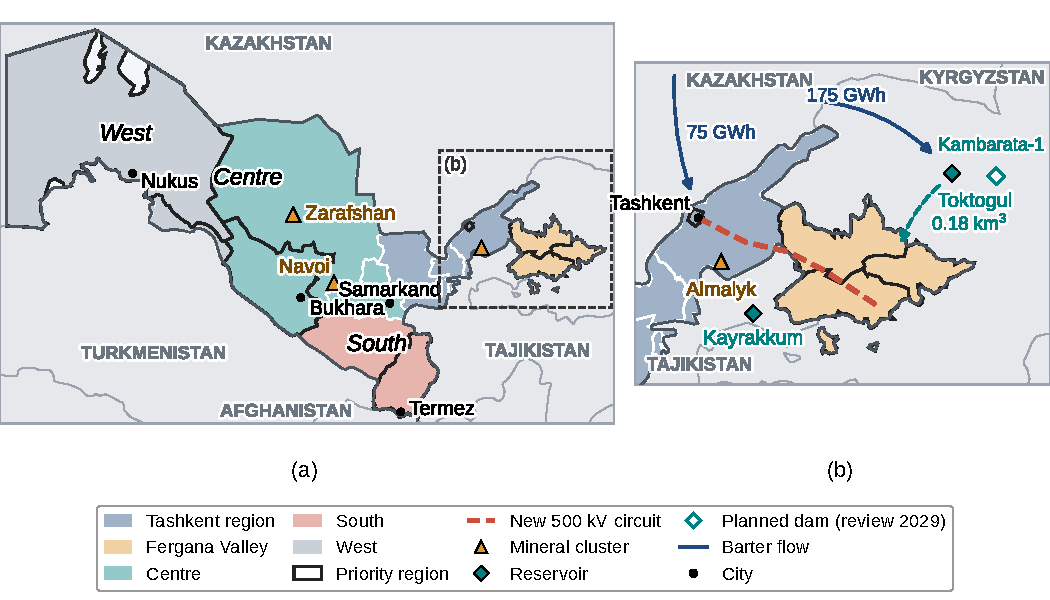
\includegraphics[width=0.85\textwidth]{figures/fig2_uzbekistan_map}
\caption{Where the plan acts. (a) The five model regions: Tashkent (city, region, Syrdarya, Jizzakh), Fergana Valley (Fergana, Andijan, Namangan), Centre (Samarkand, Navoi, Bukhara), South (Kashkadarya, Surkhandarya) and West (Karakalpakstan, Khorezm); bold outlines mark priority regions. (b) The Tashkent--Fergana area with the new 500~kV circuit, the Almalyk copper complex, the reservoirs and the barter flows. Borders: Natural Earth; provinces: Highsoft. Locations are approximate.}\label{fig:map}
\end{figure}

Shortages are a timing problem. In January 2023 Turkmen gas stopped at $-19.8\,^{\circ}$C and the country moved to rolling blackouts \cite{kun2023}; in December 2025 a turbine failure and an import cut led to 17:00--21:00 rationing until mid-January \cite{tca-rationing}. Our demand paths span the 131--154~TWh forecast for 2035 by the German Economic Team (GET) and others \cite{get-forecast}.

% =====================================================================
% 3. MODEL
% =====================================================================
\section{How we chose the investments}\label{sec:model}

We did not choose projects one at a time. Our least-cost planning model of the power and gas system follows OSeMOSYS and NEMO \cite{osemosys,nemo} and is solved in Pyomo with HiGHS \cite{team-model}. In stage 1 the government commits to what to build, where and when in 2027--2036: 16 project types, 500~kV circuits, a Kambarata-1 share (yes or no) and the barter's size. In stage 2 the system runs with whatever was built in each of twelve futures across five regions, three seasons, three parts of the day (day, the 17:00--21:00 peak, night) and a cold design day. The model minimises expected present cost $\sum_{t=2027}^{2040}(1+r)^{-(t-2027)}[\mathrm{INV}_t+\sum_\omega \pi_\omega \mathrm{OPX}_{t,\omega}]$ with $r=8\%$ and future probabilities $\pi_\omega$, within the US\$14.1 billion public budget (at most US\$2.0 billion a year), power and gas balances, regional distribution limits, build rates and lead times. Two service limits hold in expectation: unserved electricity below 2.5\% of demand in 2027--2029 and 0.44\% from 2030 (the winter 2022 and 2024 levels), and at most 1.5 million households in winter energy poverty from 2030. The model counts people, not only energy: a household is in winter energy poverty if its gas is cut, it loses evening power, or it heats with an inefficient coal or wood stove. When gas runs short, industry and CNG stations are cut first, as in January 2023 \cite{kun2023}. Reliability is a limit, not a cost, because Uzbekistan's value of lost load (US\$0.06/kWh) is too low to prevent large shortages \cite{wb2013-voll}. The futures combine demand growth of 4.8\% or 6.4\% a year, gas output that follows the official forecast (48.5~bcm by 2030) or declines 3\% a year, and normal (80\%), cold (12\%) or cold winters with an import cut (8\%) \cite{kun-target}. With the 2025 fleet the model produces 87.6~TWh against the actual 86.7~TWh. Code, inputs with sources and results: \url{https://github.com/deepshika3/oqim-uzbekistan}.

% =====================================================================
% 4. PLAN
% =====================================================================
\section{The ten-year plan}\label{sec:plan}

Table~\ref{tab:planpage} shows what the model builds and what it costs the state. Distribution upgrades take over half of the public budget; solar is financed by private producers under power purchase agreements (PPAs), and households and workover partners share the cost of boilers and wells.

\begin{table}[!t]
\centering\footnotesize
\caption{The plan by investment line. Public cost in US\$ million, undiscounted.}\label{tab:planpage}
\begin{tabularx}{\textwidth}{@{}L{0.4cm}YL{1.9cm}L{1.9cm}rrrr@{}}
\toprule
\headrow & Measure & Scale & Years & 2027--29 & 2030--32 & 2033--36 & Total \\
\midrule
P1 & Leak repair in gas networks & 1.0~bcm/yr & 2027--30 & 136 & 15 & 0 & 151 \\
P1 & Brownfield well workovers & 300 wells & 2028--33 & 122 & 365 & 122 & 609 \\
P1 & Utility solar (private, PPA) & 11.0~GW & 2031--35 & 0 & 0 & 0 & 0 \\
P1 & Small hydro (Tashkent) & 40~MW & 2027 & 58 & 0 & 0 & 58 \\
P2 & Distribution upgrades & 9.4~GW & 2027--34 & 1,687 & 661 & 463 & 2,811 \\
P2 & Tashkent--Fergana 500~kV line & 1 circuit & 2029--32 & 164 & 0 & 0 & 164 \\
P3 & Efficient gas boilers & 2.1~m homes & 2027--33 & 387 & 387 & 129 & 903 \\
P3 & Clean stoves (homes without gas) & 1.18~m homes & 2027--30 & 239 & 15 & 24 & 278 \\
P6 & Barter metering and settlement & 3 legs & 2027--36 & 40 & 4 & 6 & 50 \\
\midrule
 & \textbf{Total public} & & & \textbf{2,833} & \textbf{1,447} & \textbf{744} & \textbf{5,024} \\
\bottomrule
\end{tabularx}
\end{table}

Homes and heat come first because they reach people most cheaply. A boiler at about 80\% efficiency saves around 625~m\textsuperscript{3} of gas a winter for US\$860, and a clean stove halves solid-fuel use for US\$236 \cite{esmap-kg}. Stoves reach 1.18 million of the 2.5 million coal and wood households by 2030, and most of the 1.5 million households still counted are the rest. The cap stays at 1.5 million because stoves and boilers can only be installed so fast; reaching 1.0 million from 2032 needs 330,000 more stoves, 4~GW more distribution, gas storage and Kambarata-1, about US\$3.6 billion in our model, which is why conditional funds are released only at the 2029 and 2032 reviews (Table~\ref{tab:budget}). Leak repair and workovers add gas faster than any new field \cite{wb-gasnet}.

On the power side the binding limit is the grid. Without new projects, 2032 evening cuts reach about 810~GWh in Tashkent and 560~GWh in Fergana; distribution upgrades and the new circuit cut them to 4 and 50~GWh (Figure~\ref{fig:results}b). Solar does not cover the evening peak, but it saves daytime gas so plants can run in the evening; by 2036 solar supplies about 35~TWh and the Jizzakh nuclear plant under construction about 17~TWh \cite{wnn-nuclear}. Households in winter energy poverty fall from 2.7 million to 1.5 million by 2030 and stay there (Figure~\ref{fig:results}a). A rural Surkhandarya family on coal gets a free clean stove by 2029 through its mahalla \cite{mfa-mahalla}, halving fuel use and smoke \cite{wb-female}, while evening outages in the South fall from 540 to 20~GWh.

\begin{figure}[!t]
\centering
\begin{minipage}[b]{0.32\textwidth}\centering
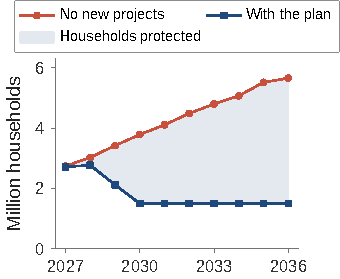
\includegraphics[max width=\linewidth]{figures/fig5a_households}\\[-2pt]{\small (a)}
\end{minipage}\hfill
\begin{minipage}[b]{0.32\textwidth}\centering
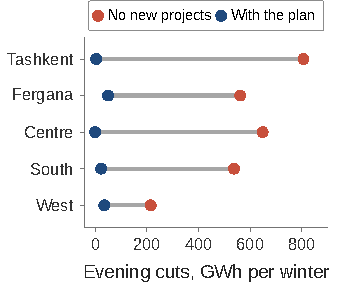
\includegraphics[max width=\linewidth]{figures/fig5b_regional_cuts}\\[-2pt]{\small (b)}
\end{minipage}\hfill
\begin{minipage}[b]{0.32\textwidth}\centering
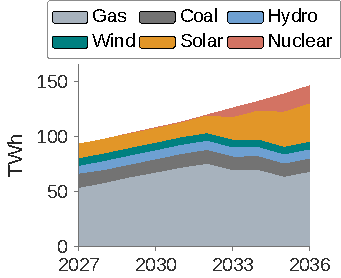
\includegraphics[max width=\linewidth]{figures/fig5c_generation_mix}\\[-2pt]{\small (c)}
\end{minipage}
\caption{Model results, expected over the twelve futures \cite{team-model}. (a) Households in winter energy poverty. (b) Winter evening cuts (17:00--21:00) by region in 2032. (c) Generation with the plan; about 2~TWh of imports a year not shown.}\label{fig:results}
\end{figure}

Table~\ref{tab:mix} explains the mix. Solar adds 11~GW but nothing at the winter evening peak, so firm capacity comes from committed gas plants and nuclear; in 2036 accredited capacity is only about 1~GW above the expected peak, and it depends on gas, so the plan buys gas security first. The model rejected wind (15\% credit at the peak) \cite{ns-bash}, plant rebuilds, insulation (US\$9,300 a home) \cite{wb-heating} and pump upgrades. Batteries enter only below about US\$35/kWh for a two-hour system, a fifth of today's US\$165, because evening shortages come from grid limits and gas. Kambarata-1 is not chosen in the standard runs and is reviewed in 2029.

\begin{table}[!t]
\centering\footnotesize
\caption{Generation mix, 2025 and 2036 with the plan. Accredited capacity is what counts at the 17:00--21:00 winter peak.}\label{tab:mix}
\setlength{\tabcolsep}{4pt}
\begin{tabularx}{\textwidth}{@{}Yrrrrrr@{}}
\toprule
\headrow Source & GW 2025 & GW 2036 & Peak credit & Accredited 2025 & Accredited 2036 & TWh 2036 \\
\midrule
Old gas steam units & 8.2 & 8.2 & 0.75 & 6.1 & 6.1 & 13.3 \\
Combined-cycle gas and engines & 6.9 & 11.1 & 0.90 & 6.2 & 10.0 & 53.7 \\
Coal (Angren) & 2.5 & 2.5 & 0.75 & 1.9 & 1.9 & 12.1 \\
Hydro (incl.\ Pskem, small hydro) & 2.4 & 2.9 & 0.80 & 1.9 & 2.3 & 8.3 \\
Solar & 3.9 & 17.9 & 0 & 0 & 0 & 34.8 \\
Wind & 2.1 & 2.1 & 0.15 & 0.3 & 0.3 & 6.9 \\
Batteries (2-hour) & 2.4 & 2.4 & 0.50 & 1.2 & 1.2 & -- \\
Nuclear (Jizzakh) & 0 & 2.1 & 0.90 & 0 & 1.9 & 16.6 \\
\midrule
\textbf{Total} (expected peak 13.2~GW in 2025, 22.8~GW in 2036) & \textbf{28.4} & \textbf{49.2} & & \textbf{17.6} & \textbf{23.7} & \textbf{145.7} \\
\bottomrule
\end{tabularx}
\end{table}

% =====================================================================
% 5. IMPACT
% =====================================================================
\section{Impact on the economy, households and environment}\label{sec:impact}

\textit{Economy.} The plan cuts gas imports by 9.7~bcm over 2027--2036, about US\$1.6 billion at the US\$160 per 1,000~m\textsuperscript{3} paid for Russian gas \cite{kun-gazprom}, and avoids 15~bcm of expected gas cuts to industry and CNG stations, protecting fertiliser, chemicals, metals and transport fuel in cold winters. Unserved electricity falls by 2.9~TWh in 2030 and 7.1~TWh in 2032. Jobs from installing 3.3 million boilers and stoves are tracked, not assumed.

\textit{Household bills.} Since 1 June 2026, 300~kWh a month costs UZS~220,000 (UZS~650/kWh to 200~kWh, 900 above), and gas costs UZS~1,100/m\textsuperscript{3} within the 500~m\textsuperscript{3} winter norm and 2,000 above \cite{moe-tariff,kun-tariff2026}; the October 2026 changes are proposed, not enacted, and not assumed \cite{moe-proposals}. A household pays half of a US\$860 boiler, about UZS~5.1 million at UZS~12,000 per dollar \cite{zamin-fx}, and saves UZS~0.7--1.25 million a winter, a payback of four to eight winters. Stoves are free to eligible families and halve their coal or wood spending. Compensation (UZS~1 million a year) \cite{wb-reforms} and efficiency keep a basic package below 5\% of spending.

\textit{Environment, including the costs.} Power-sector CO\textsubscript{2} is 41~Mt in 2036 with the plan against 46~Mt without new projects, and repairing 1.0~bcm a year of leaks avoids about 21~Mt~CO\textsubscript{2}e a year if that gas would otherwise vent (methane at 29.8 times CO\textsubscript{2}) \cite{ipcc-ar6}. There are negatives. Solar needs about 22,000~ha; the model sites it in the Centre, South and Tashkent on non-irrigated land, with dry cleaning and planted dust buffers, with none in Karakalpakstan without a dust and habitat review. Toktogul's summer releases change river flows, so they stay above ecological minimums and shrink in dry years. And 2.1 million gas boilers lock in gas heating to about 2042, so they must have low-NO\textsubscript{x} burners and be heat-pump-ready, and public boiler subsidies end after 2033. \textit{Social effects.} Clinics, schools and water and wastewater pumps sit on priority feeders and are tracked by outage hours; barter water is reported as water received by each irrigation area; avoided gas cuts keep CNG stations open; and clean stoves cut the time, mostly women's, spent gathering fuel and breathing smoke.


\noindent\fcolorbox{headblue}{rowblue!40}{\parbox{\dimexpr\linewidth-2\fboxsep-2\fboxrule}{\footnotesize\textbf{How the headline numbers are derived.} Saving: present cost 2027--2040 at 8\% is US\$30,240~million with no new projects and US\$28,124~million with the plan, a difference of US\$2.1~billion \cite{team-model}. Unserved electricity: 3.39 $-$ 0.49 = 2.9~TWh (2030); 7.65 $-$ 0.54 = 7.1~TWh (2032). Imports: 79.5 $-$ 69.8 = 9.7~bcm. Heat losses falling from 38\% to 20\% cut the input for the same useful heat by 1 $-$ 0.62/0.80 = 22.5\%. Solar: IRENA's US\$691/kW for 2024 \cite{irena}, falling 4.7\% a year, gives US\$410--490/kW in 2031--2035, in line with Uzbek auctions under 2~US\textcent/kWh \cite{mercom-masdar}, so 11~GW costs about US\$4.9~billion.}}

% =====================================================================
% 6. STRESS TESTS
% =====================================================================
\section{Stress tests}\label{sec:stress}

A plan designed for the average future cannot reach the 1.5 million target (its best is 1.83 million), and perfect foresight would be worth about US\$1.5 billion, so the plan favours fast, flexible measures early. Across nine tests (discount rates, outage and gas-shortage values, late nuclear, weaker lines, less available plants, faster gas decline, no barter) public spend stays between US\$4.6 and 6.2 billion and the core measures are always chosen; gas storage enters only when gas shortages are valued twice as high or money is cheaper (6\%) \cite{team-model}. A one-year slip of every project costs US\$1.8 billion and moves the target to 2031, and a two-year slip makes it unreachable, hence the readiness gate. Gas cuts to industry still reach 4.5~bcm in 2036, so industrial efficiency and storage are reviewed in 2029.

% =====================================================================
% 7. BARTER
% =====================================================================
\section{Barter partnership: seasonal water--energy exchange}\label{sec:barter}

The barter buys what Uzbekistan cannot build in time: firm winter-evening power and growing-season water from the Naryn cascade. Kazakhstan supplies winter power to Kyrgyzstan and Uzbekistan; Uzbekistan repays Kazakhstan with summer solar-hour power; and Kyrgyzstan keeps water in Toktogul instead of generating with it in winter, repaying Uzbekistan with summer hydropower and an extra July--August release (Figure~\ref{fig:barter}). Kazakhstan needs summer power in its south \cite{astana2025}; Kyrgyzstan owns Toktogul and imported 3.6~TWh in 2024 \cite{tca2025}; Tajikistan is the drought contingency via Kayrakkum and the Regar--Guzar line. Turkmenistan has no seasonal storage and Afghanistan no winter surplus. The 1998 Syr Darya Agreement lapsed after 2002 and the 2025 protocols have no repayment rule \cite{syr1998,astana2025}, so the three ministries sign a new protocol (Table~\ref{tab:terms}) with a Tajik annex.

\begin{figure}[!t]
\centering
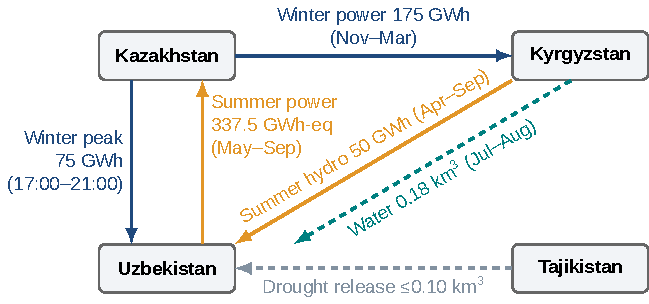
\includegraphics[width=0.52\linewidth]{figures/fig7a_barter_legs}
\caption{The three legs of the exchange per annual cycle; blue winter power, amber summer power, teal water, grey the drought contingency.}\label{fig:barter}
\end{figure}

Settlement uses one unit: 1~GWh-eq is 1~GWh of summer-window power, and winter deliveries count 1.35 times. Kazakhstan delivers (175 + 75)~GWh $\times$ 1.35 = 337.5~GWh-eq, settled by Uzbekistan's summer delivery. Uzbekistan finances 175 $\times$ 1.35 = 236.25~GWh-eq for Kyrgyzstan, repaid by 50~GWh of summer hydro and about 0.18~km\textsuperscript{3} of extra release valued at 186.25~GWh-eq; at 0.9--1.0~kWh per m\textsuperscript{3} on the cascade, 175~GWh of avoided winter generation leaves about 0.18~km\textsuperscript{3} in Toktogul \cite{usaid-epic}. Kyrgyzstan is paid once, with 175~GWh of winter power; the water credit only repays Uzbekistan for financing it. The cascade output from the release is the same water's energy moved from winter to summer, when Kyrgyz power is worth least, so Kyrgyzstan keeps it and it is credited to no account.

\begin{table}[!t]
\centering\footnotesize
\caption{Contract term sheet, per annual cycle.}\label{tab:terms}
\begin{tabularx}{\textwidth}{@{}L{3.0cm}L{1.5cm}L{2.8cm}L{2.3cm}Y@{}}
\toprule
\headrow Obligation & Quantity & Window, maximum rate & Measured at & Consideration \\
\midrule
Kazakh winter power to Kyrgyzstan & 175~GWh & Nov--Mar, 24~h; $\le$50~MW & Kazakh--Kyrgyz border & Paid by Uzbekistan: 236.25~GWh-eq \\
Kazakh peak power to Uzbekistan & 75~GWh & 120 days, 17:00--21:00; $\le$160~MW & Kazakh--Uzbek border & 101.25~GWh-eq \\
Uzbek summer power to Kazakhstan & 337.5~GWh-eq & May--Sep, 8-h windows; $\le$280~MW & Kazakh--Uzbek border & Settles both Kazakh deliveries \\
Kyrgyz summer hydro to Uzbekistan & 50~GWh & Apr--Sep; $\le$35~MW & Kyrgyz--Uzbek border & 50~GWh-eq \\
Kyrgyz extra release & $\approx$0.18~km\textsuperscript{3} & Jul--Aug; $\approx$34~m\textsuperscript{3}/s & Uchkurgan; canal heads & 186.25~GWh-eq \\
Tajik contingency release & $\le$0.10~km\textsuperscript{3} & Jul--Aug, drought only & Kayrakkum outflow & Uzbek power, $\le$1.0~kWh-eq/m\textsuperscript{3} \\
\bottomrule
\end{tabularx}
\end{table}

Until the plan's solar arrives in 2031, Uzbekistan repays from its existing and committed solar (about 6.9~GW), under 5\% of its May--September output. Kazakhstan is a net importer over a year (2.4~TWh short in 2024) \cite{timesca-kzdeficit}, so firmness is not assumed: 250~GWh is 0.2\% of its generation, capacity is reserved and tested before each season, and a failed test means the leg is not activated and nothing is owed. The 75~GWh is a pilot, about 5\% of the 1,370~GWh of modelled 2032 evening cuts in Tashkent and Fergana without new projects; domestic upgrades close the rest. A Joint Settlement Committee recalibrates the 1.35 coefficient each September within 1.2--1.5; Energiya schedules flows \cite{cdc-energiya}, the Basin Water Organisation (BWO) Syrdarya verifies releases, and meter data are shared in real time.

Shortfalls below 95\% of a monthly contract are made up within 60 days at 110\%; notified maintenance, grid-security curtailment and force majeure are excused; low inflow scales the Kyrgyz release and activates the Tajik annex; two unexcused shortfalls suspend the leg; disputes go to the Committee, the independent engineer, then UNCITRAL arbitration. Each cycle is judged on energy delivered (at least 95\%), water received by each irrigation area (at least 90\%), no evening rationing on priority feeders, reported feeder by feeder, and equipment accepted. The pilot needs US\$50 million for metering and verification. At the 2029 review it may double from 2030 only after two verified cycles with net benefit for every party, and any party may exit with 12 months' notice once balances are settled. Winter shortages make the pilot welcome in Kyrgyzstan, and it does not depend on Kambarata-1. In the model it is about cost-neutral for Uzbekistan and adds 160~MW of firm evening supply, a first step towards integration worth US\$3.5 billion a year \cite{agora}.

% =====================================================================
% 8. DELIVERY
% =====================================================================
\section{Delivering the plan}\label{sec:delivery}

The Ministry of Energy owns delivery through one project unit, working with the National Electric Grid, the regional distribution companies and Uztransgaz; the Ministry of Economy and Finance releases money, holds the reserve and records PPP obligations as contingent liabilities \cite{imf-2026}; an independent engineer signs baselines and acceptance; and the regulator sets tariffs and standards \cite{emdra}. Every project passes a readiness gate (permits, grid connection, offtake, funded maintenance), and every contract names the owner, the operator and who pays for maintenance.

\textit{CESAN} builds on unbundling, bilateral-contract rules and the Samarkand distribution PPP \cite{samarkand-ppp,team-cesan}. It ties network spending to audited feeder performance, choosing per district between public delivery, a performance contract or a concession, and opens industrial bilateral contracts. The US\$400 million envelope (US\$360 million public, including a US\$180 million network line, and US\$40 million private) breaks even at 18~GWh a year of avoided outages \cite{wb-pad}; the plan avoids 2.9~TWh in 2030, so the hurdle is small, but CESAN's own share is proven against matched untreated feeders. Delhi and Uganda show both the gain and the need for fixed exit terms \cite{tata-delhi,umeme}.

\textit{The mineral--energy compact} links Uzbekistan's 120 planned mineral projects \cite{pres-minerals} to the grid: a mine shares a substation with nearby mahallas only if sharing is cheaper than separate connections \cite{columbia-shared}, and a copper-to-grid programme qualifies Uzbek cables and transformers \cite{iea-minerals}. Other projects proceed only after site audits, learning from Hamburg and Chile. Its US\$540 million envelope holds US\$390 million of base capital (shared grids 180, equipment 55, efficiency and heat 80, battery pilot and critical-service solar 60, preparation 15); sponsors provide US\$280 million and US\$200 million is public, led by Almalyk \cite{team-minerals}.

\textit{Communities.} Mahalla committees choose the families who receive boilers and stoves against published criteria, and Inson social-service centres handle enrolment and complaints \cite{wb-inson}; a complaint goes to the mahalla, then the Inson centre (answer within 15 days), then the independent engineer. Consultation and an environmental and social assessment precede the Tashkent--Fergana route and any mine-adjacent works.

\textit{Operation and maintenance.} The portfolio needs about US\$70 million a year once built, mostly 2\% a year on distribution, paid from tariffs through an escrow released only against audited maintenance, which lifts distribution's revenue share from 11\% towards 20--30\% \cite{wb-p504630}. After the December 2025 turbine failure, the 8.2~GW of old steam units get an overhaul each April--May, paid from the reserve.

\noindent\fcolorbox{headblue}{rowblue!40}{\parbox{\dimexpr\linewidth-2\fboxsep-2\fboxrule}{\footnotesize\textbf{The first 180 days.} \textit{Days 1--30:} Cabinet adopts the plan; project unit, budget line, reserve rules and independent engineer in place. \textit{Days 31--90:} mahalla and Inson enrolment opens; leak-repair and workover tenders; feeder outage baselines measured; barter heads of terms signed and Kazakh capacity tested. \textit{Days 91--180:} first boilers and stoves installed; Tashkent--Fergana route consultation; first solar auction announced; O\&M escrow set up; first quarterly public report.}}

% =====================================================================
% 9. FINANCING
% =====================================================================
\section{Targets, financing and roadblocks}\label{sec:financing}

The programme assigns the full US\$14.102 billion public ceiling (Table~\ref{tab:budget}): US\$10.150 billion of base investment, US\$2.450 billion of conditional expansion and a US\$1.502 billion emergency reserve. Domestic budget provides US\$10.352 billion and development banks US\$3.750 billion, with the World Bank, ADB, EBRD, AIIB and IsDB the first lenders to approach. The model's core portfolio (US\$5.0 billion, Table~\ref{tab:planpage}) sits within the base. Private capital sits outside the ceiling: the initial US\$12.630 billion pipeline, mostly renewables and storage under PPAs, brings total mobilisation to US\$26.732 billion; spread over ten years it stays within the IMF's US\$6.5 billion annual PPP cap if obligations are disclosed and tariffs auctioned \cite{imf-2026}. Conditional funds are released only by the December 2029 and December 2032 reviews.

\begin{table}[!t]
\centering\footnotesize
\caption{OQIM financing plan (US\$ billion, constant 2025)}\label{tab:budget}
\setlength{\tabcolsep}{3.5pt}
\begin{tabularx}{\textwidth}{@{}Y rrr rrr rr@{}}
\toprule
 & \multicolumn{3}{c}{Public sources} & \multicolumn{3}{c}{Public max., of which} & & \\
\cmidrule(lr){2-4}\cmidrule(lr){5-7}
Investment package & Domestic & MDB & Public max. & Base & Dec 2029 & Dec 2032 & Private & Total mobilised\\
\midrule
\multicolumn{9}{@{}l}{\textit{Investment packages}}\\
Networks and metering              & 1.660 & 2.250 & 3.910 & 2.710 & 0.700 & 0.500 & --     & 3.910\\
Gas recovery and delivery          & 1.600 & --    & 1.600 & 1.200 & 0.400 & --    & 1.350  & 2.950\\
Renewables and storage             & 1.020 & --    & 1.020 & 0.520 & --    & 0.500 & 10.150 & 11.170\\
Irrigation                         & 0.600 & 0.900 & 1.500 & 1.150 & --    & 0.350 & --     & 1.500\\
Heating and industry               & 1.450 & 0.300 & 1.750 & 1.750 & --    & --    & 1.130  & 2.880\\
District heat efficiency           & 0.200 & 0.300 & 0.500 & 0.500 & --    & --    & --     & 0.500\\
Critical-facility resilience       & 0.270 & --    & 0.270 & 0.270 & --    & --    & --     & 0.270\\
Regional exchange and hydro option & 0.600 & --    & 0.600 & 0.600 & --    & --    & --     & 0.600\\
\cmidrule(l){2-9}
\textit{Subtotal}                  & 7.400 & 3.750 & 11.150 & 8.700 & 1.100 & 1.350 & 12.630 & 23.780\\
\multicolumn{9}{@{}l}{\textit{Delivery and risk buffers}}\\
Delivery and verification          & 0.450 & --    & 0.450 & 0.450 & --    & --    & --     & 0.450\\
Cost-uncertainty allowance         & 1.000 & --    & 1.000 & 1.000 & --    & --    & --     & 1.000\\
Emergency reserve$^{a}$            & 1.502 & --    & 1.502 & --    & --    & --    & --     & 1.502\\
\midrule
\textbf{Total} & \textbf{10.352} & \textbf{3.750} & \textbf{14.102} & \textbf{10.150} & \textbf{1.100} & \textbf{1.350} & \textbf{12.630} & \textbf{26.732}\\
\bottomrule
\end{tabularx}
\par\smallskip{\scriptsize\raggedright \textit{Assumptions.} (i) Constant 2025 US\$; private capital sits outside the public ceiling. (ii) Development banks (MDB) co-finance only lines with an existing bank programme (networks, irrigation, heating, district heat); all other lines are domestic. (iii) Base funds cover the model's core portfolio (US\$5.0 billion, Table~\ref{tab:planpage}) plus planning allowances for lines the model does not size (irrigation, district heat, critical facilities, delivery and verification). (iv) Dec 2029 and Dec 2032 funds are released only if that review confirms the trigger (stricter household or reliability target, gas decline, verified delivery). $^{a}$\,Held outside base and conditional funding: US\$0.450B operator step-in, US\$0.400B seasonal backup, US\$0.250B winter lifeline support, US\$0.402B residual risks.\par}
\end{table}


Build rates match recent experience \cite{enerdata}. Technologies not chosen today are watched with a trigger each. Batteries return below about US\$35/kWh or after two good winters in the compact's cold-weather pilot. Heat pumps save gas only above a coefficient of performance (COP) of 1.95--3.04 against an 85\% boiler, so they wait until the winter margin plant is over 50\% efficient and measured seasonal COP exceeds 3. Geothermal waits for wells that beat gas boilers, hydrogen for electrolysis cheaper than gas-based ammonia.

% =====================================================================
% 10. METRICS
% =====================================================================
\section{Measuring success and failure}\label{sec:metrics}

Table~\ref{tab:metrics} ties each metric to a diagnosed constraint. Outages are reported feeder by feeder and barter water by irrigation area. Milestones: 0.9 million boilers and 1.0 million stoves by 2030, the Fergana line in 2032, 11~GW of new solar by 2036. Success means verified service, not contracted capacity.

\begin{table}[!t]
\centering\footnotesize
\caption{Metrics by factor.}\label{tab:metrics}
\begin{tabularx}{\textwidth}{@{}L{2.0cm}YL{4.4cm}L{1.5cm}@{}}
\toprule
\headrow Factor & Measure & Baseline $\rightarrow$ target & Source \\
\midrule
Accessibility & Households in winter energy poverty; hours $\ge$18\,$^{\circ}$C indoors \cite{who-housing} & 2.7~m (2027) $\rightarrow$ $\le$1.5~m from 2030 & Model; survey \\
Reliability & Unserved electricity; outage duration (SAIDI) and frequency (SAIFI) \cite{ieee1366} & $\le$0.44\% from 2030; Fergana 562 $\rightarrow$ 50~GWh & Model; dispatch \\
Quality & Network losses; voltage compliance & 17.2\% $\rightarrow$ 13.4\% (2036) & Model; ministry \\
Security & Gas imports; firm supply against peak; N$-$1 adequacy (survives losing the largest unit) \cite{iea-kgz} & 9.7~bcm less imported gas & Model; Uztransgaz \\
Affordability & All-fuel spending share; arrears; under-heating & 562,918 compensated; 300~kWh costs UZS~220,000 a month (2026) $\rightarrow$ basic package ${<}$5\% of spending \cite{esmap-mtf} & Field \\
Safety & CO poisonings; electrical fires; safety checks & 125 CO deaths (2021) \cite{kun-co2021} $\rightarrow$ none in upgraded homes; 100\% checks & Field \\
Environment & Leaks repaired; absolute CO\textsubscript{2}; PM\textsubscript{2.5} \cite{who-air} & 1.0~bcm/yr by 2031; Tashkent 38.8 $\rightarrow$ 5~\textmu g/m\textsuperscript{3} & Model; field \\
Roadblocks & Readiness-gate pass rate; tenders; PPP liabilities disclosed & 100\% pass before award & Records \\
\bottomrule
\end{tabularx}
\end{table}

\FloatBarrier
% =====================================================================
{\setlength{\columnsep}{10pt}\begin{multicols}{3}
\scriptsize\setlength{\bibsep}{0pt}
\bibliographystyle{unsrtnat}
\bibliography{refs}
\end{multicols}}

\end{document}
